\section{Concepts of Co-Evolutionary Testing}
\label{testing}
Learning systems are often used in safety critical domains, where potential failures can have catastrophic consequences. Therefore, it is essential to evaluate said architectures thoroughly to minimize risk and maximize safety. Due to their limitations, traditional random testing algorithms cannot ensure minimum failure probability (see \ref{limitations}). To address this issue, the following chapter focuses on concepts of co-evolutionary testing. Section \ref{avf} and \ref{coevolution} including their subsections will describe and section \ref{comparison} will assess two state of the art co-evolutionary evaluation methods.

%----------Problem-------------

\subsection{Limitations Of Random Testing}
\label{limitations}
As mentioned before, a thorough testing process is necessary before integrating the learning system in a safety critical domain. When using a traditional random testing algorithm, usually the confidence that the failure rate of a policy is below $\epsilon$ requires at least $1/\epsilon$ testing episodes. This might be inefficient and time-intensive. For example in a autonomous driving domain. If there is a greater failure probability than $\epsilon = 10^{-8}$ per mile, meaning the car would crash at least once in 100 million miles, it would not be brought on the market. In order to achieve reasonable confidence, the manufacturer would need to test-drive the car for at least $10^{-8}$ miles, which may be prohibitively expensive \cite{uesato18}. Additionally, we don't exactly know how the environment will behave unless all possibilities are tried. For a huge variety of scenarios this process can get unreasonable. The agent can be trained and tested on random samples from the scenario space. However, this might cause the agent to specialize on the average scenario, which might provoke incidents. Hence, the agent is still not fully dependable \cite{gabor19}. To overcome these obstacles, a novel testing approach is needed.

\subsubsection{Intelligence Tests}
\label{intelligence}
Hernández-Orallo \& Dowe \cite{orallo10} introduced the \textit{anytime intelligence test}. This test adapts to the current intelligence of the system. When the systems' intelligence changes, the test adjusts itself. The basic idea is to initially test the agent on easy levels. When the agent succeeds it needs to overcome a harder environment. A set of environments of different complexity is required to evaluate the agent. These environments were created on a theoretical base (e.g. Solomonoff prediction) with a determined a priori complexity. This approach tests the intelligence of a system, but can not thoroughly test a learning system. The autonomous car, for example, still needs to see a unreasonable amount of scenarios.\\
Insa-Cabrera et al. \cite{cabrera11} used the idea of \cite{orallo10} to construct a general intelligence test for the evaluation of reinforcement learning algorithms. Here, all possible environments are ordered by their Kolmogorov complexity from which a set of samples is drawn. With this set, adaptive tests can be constructed which can be used to evaluate an agent. However, this concept only examines well-known properties of Q-learning. It is not known if this method works for other reinforcement learning algorithms, too. The problem, that all possible environments are needed, still exists.

\subsubsection{Co-Evolution}
\label{coevolutio}
Gabor et al. \cite{gabor18} claim that all steps related to testing adaptive systems need to become self-adaptive. In order to achieve adaptive quality assurance, they introduced the paradigm of scenario coevolution. Instead of randomly creating test scenarios, this architecture describes a set of test cases, that evolves in parallel to the behavior of the system. In this publication, the co-evolutionary process is applied to software engineering, where the test wants to find bad behavior in the productive code, whereas the productive code tries to avoid making mistakes.\\
The testing algorithm and the productive code competitively co-evolve. Wang et al. \cite{wang19} used this concept to generate increasingly complex and diverse learning environments through evolutionary strategies. They train a neural network controlling a walker that tries to optimize for an environment. These environments can be modified by the algorithm (POET - \textbf{P}aired \textbf{O}pen-\textbf{E}nded \textbf{T}railblazer) to create increasingly complex scenarios, the agent needs to solve. This way, POET managed to produce a diverse range of highly developed behaviors for a big range of environments. Unfortunately, this concept can only be used to train the agent. The testing problem still exists.\\
Co-evolutionary approaches in training help the agent to minimize failures. Therefore, it may seem obvious, that co-evolutionary techniques can be used for an efficient evaluation of reinforcement learning systems.

%----------Evaluation-------------

\subsection{Failure Probability Predictor (AVF)}
\label{avf}
Uesato et al. \cite{uesato18} proposed a failure probability predictor (AVF) for evaluating learning systems. If not stated otherwise, this chapter derives from the original paper. This architecture follows two specific tasks. To find a catastrophic failure of the agent (see section \ref{failure}) and to estimate the \textit{failure probability} up to a fixed \textit{relative accuracy} with high probability of given failure (see section \ref{risk}).\\
On both objectives, the algorithm has access to historical data and can sample from the distribution $P_X$ over initial states $X$ defined by the environment.\\
The AVF $f_*:X->[0,1]$ returns the probability of a failure given a initial condition. The estimators were assessed by the total number of experiments required and compared with 
the \textit{vanilla Monte Carlo} estimator (VMC).

\subsubsection{Failure Search}
\label{failure}


\subsubsection{Risk Estimation}
\label{risk}


%----------Concepts Of Scenario Co-Evolution-------------

\subsection{Scenario Co-Evolution}
\label{coevolution}
The Scenario Co-Evolution method by Gabor et al. \cite{gabor19} is another novel approach to tackle the issue of testing learning systems reliably. If not stated otherwise the content of this chapter derives from the original publication.\\
This concept is an instance of the general architecture of \cite{gabor18} briefly mentioned in section \ref{limitations}. The basic idea is to train an evolutionary algorithm, that co-evolves with a reinforcement learning agent and actively finds problems that are hard to solve for the agent. While the expertise of the agent evolves, the set of test instances (or \textit{scenarios}) co-evolves. After training, the co-evolutionary algorithm should return a set of hard test scenarios, that can be used for evaluating the agent.\\\\
More specifically, hard settings $x$ (or values $x$) from the scenario space $\chi$, for which the agents' performance deteriorates are wanted. Similar to Zero-sum Markov games (section \ref{zerosumgames}) two algorithms optimize against each other. While the agent tries to maximize its fitness, the co-evolutionary algorithm tries to find scenarios which minimize the agents' fitness. An evolutionary algorithm (section \ref{evolutionaryalgorithms}) that optimizes for hard settings for $x$ is used to find those the respective values for $x$. Figure \ref{fig:scenario_coevolution} shows a visual representation of the evolutionary algorithm.
\begin{figure}
  \centering
  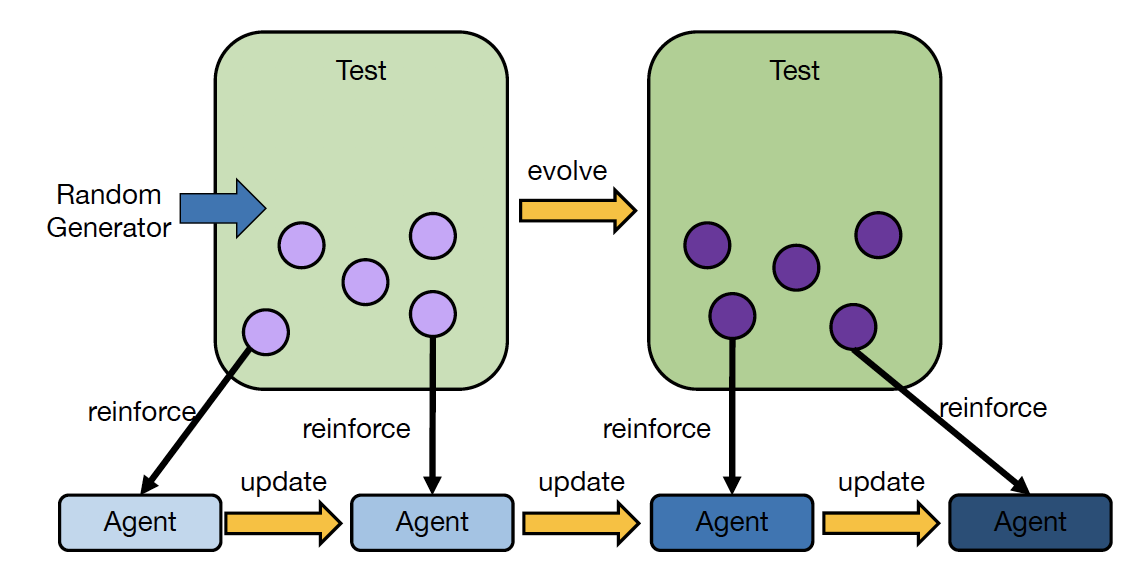
\includegraphics[width=0.85\textwidth]{adversarial_learning/images/scenario_coevolution.png}
  \label{fig:scenario_coevolution}
  \caption{Visual representation of the evolutionary process by \cite{gabor19}. First, a set of test scenarios is randomly generated. The set improves via evolution. Between evolution steps, the test data is used to train the agent. This causes the reinforcement learning agent to co-evolve with the test data.}
\end{figure}
It constructs an evolutionary process with the scenario space $\chi$. Experience samples are needed to train the agent. These are drawn using settings for $x \in \chi$ from the current population $\chi$ of the evolutionary process. After all $x \in \chi$ have been used, the evolutionary process evolves further for a few generations. In this work, the evolutionary step function for selection schemes $\sigma_1, \sigma_2, \sigma_3$ is:
\begin{equation}
X_{i+1} = o(X_i) = sel(mig_{\sigma_3}(mut_{\sigma_2}(rec_{\sigma_1}(X_i))),|X_i|)
\end{equation}
After a few generations of optimizing for hard $x$ the resulting experience sample is used to generate experience samples for the reinforcement learning agent. As mentioned, the reinforcement learning agent tries to maximize its reward, while the evolutionary process tries to minimize the fitness. The fitness $f(x)$ assigned to each $x \in \chi$ is calculated using the accumulated reward of running the current agent policy $\pi$ on the MDP $M_x$ (section \ref{mdp}). In turn, the reinforcement learning agent with the current highest fitness score is used to evaluate the hardness of the settings for $x$ for the next few generations of evolution.\\
With every evolutionary step the agent trains on harder settings from the test population. Simultaneously the fittest agent evaluates the hardness of the settings. In the end, the algorithm is able to return a set with the hardest test scenarios. When the agent can solve these hard problems, it can be assumed that it can solve easy scenarios, too. Consequently, there is no need to generate all possible scenarios. Additionally, these scenarios are not limited to the trained agent. They can be used to evaluate every agent running on the same environment.

\subsection{Comparison}
\label{comparison}
This chapter compares the \textit{failure probability predictor} (AVF) (section \ref{avf}) and the \textit{Scenario Co-Evolution} (SCoE) (section \ref{coevolution}) testing approaches. The goal of each concept is to outperform standard evaluation approaches for reinforcement learning agents by finding a more efficient method of detecting rare, catastrophic failures. While the AVF uses \textit{importance sampling} to actively search for failures and estimate the failure risk, the SCoE uses \textit{evolutionary algorithms} to evolve a set of hard test scenarios to evaluate the agent. While both architectures outperform traditional random testing methods and solve the problem of having to test the agent on every scenario, they are fundamentally different.\\\\
Both algorithms co-evolve with an agent. Because the AVF looks for failures of this specific agent, it specializes on it. Meaning, the testing algorithm cannot be used to evaluate another, independently trained agent running on the same domain.\\
SCoE however does just that. The resulting test scenarios of the SCoE are hard to solve for any other agent. Once the SCoE returns a set of test scenarios, all agents running on the same environment can be evaluated with this exact set. SCoE is a more generic and simpler way to test agents on a specific domain.\\\\
A standard random reinforcement learning agent performs worse on SCoE generated scenarios than on random generated scenarios. It shows that SCoE generated scenarios discover more catastrophic failures than traditional generated scenarios. Hence, the SCoE testing process is more reliable. Still, we simply assume, that the agent can solve easy scenarios, if it is able to overcome hard cases. The agent gets better in all scenarios by training on hard scenarios, but still does not explicitly look for failures like the AVF.\\
As already described, the AVF actively searches for failures of the agent. In comparison to a standard \textit{Vanilla Monte Carlo} (VMC) estimator, the AVF minimizes the errors in risk estimation in a fraction of the time. For example, the VMC needs 12000 episodes in a driving domain whereas the AVF minimizes the errors in risk estimation after only 2000 episodes. Additionally, the error rate of the AVF is smaller after 2000 episodes, than the VMCs error rate ever is. Unfortunately, there is no measurement of the error rate for the SCoE. Because the AVF actively searches for failures while the SCoE "only" provides hard test cases, it might lead to the assumption, that the AVF is less error-prone.\\\\
Optimization through evolutionary algorithms tend to be slow for computationally intensive problems regarding the evaluation of each problem \cite{cruz}. Importance Sampling is often used to produce fast learning algorithms \cite{chen18, schaal04}. The underlying search algorithms lead to the supposition, that AVF (with Importance Sampling) might faster per timestep than SCoE (with Evolutionary Algorithms). Unfortunately, there is no direct comparison possible.\\\\
The SCoE was used to train and test an agent trying to transport items to workstations in a comprehensible multi-agent $7 \times 8$ grid \textit{smart factory domain}. The AVF was evaluated in a continuous \textit{driving} domain, where the agent was rewarded for forward progress without crashing and in a continuous \textit{humanoid} domain, where the agent was rewarded for standing without falling. It is not known, how the AVF performs in a multi-agent domain and vice versa. At this point, we can not know, which method is a better fit for a specific type of environment.\\\\
In summary, the SCoE is a more intuitive approach, can evaluate independent agents and is proven to work great in small grid domains. The AVF might be more reliable, reduces time of searching for failures, but specializes in one agent.